%\documentclass[fleqn, letterpaper]{amsart}
\documentclass[fleqn, letterpaper]{tufte-handout}
\usepackage{times}
\usepackage{amsmath}
\usepackage{graphicx}
\usepackage{booktabs}
\usepackage{multirow}
\usepackage{listings}
\usepackage{epstopdf}
%\usepackage[left=1in]{geometry}

\newcommand{\R}{\mathcal{R}}
\newcommand{\E}{\text{E}}
\newcommand{\p}{p_{XY}}
\renewcommand{\arraystretch}{1.5}

\title{Problem Set 4 --- ENCE689E Spring 2014}
\author{David Prentiss}

\begin{document}
\maketitle

\section{Time-varying (Dynamic) Model}
\subsection{(a)}
\subsection{(a)}
\subsection{(a)}
\subsection{(a)}
\subsection{(a)}
\subsection{(a)}
\[z = \alpha_1x_1^2+\alpha_2x_2^2 = Ax\]
where 
\begin{figure}
        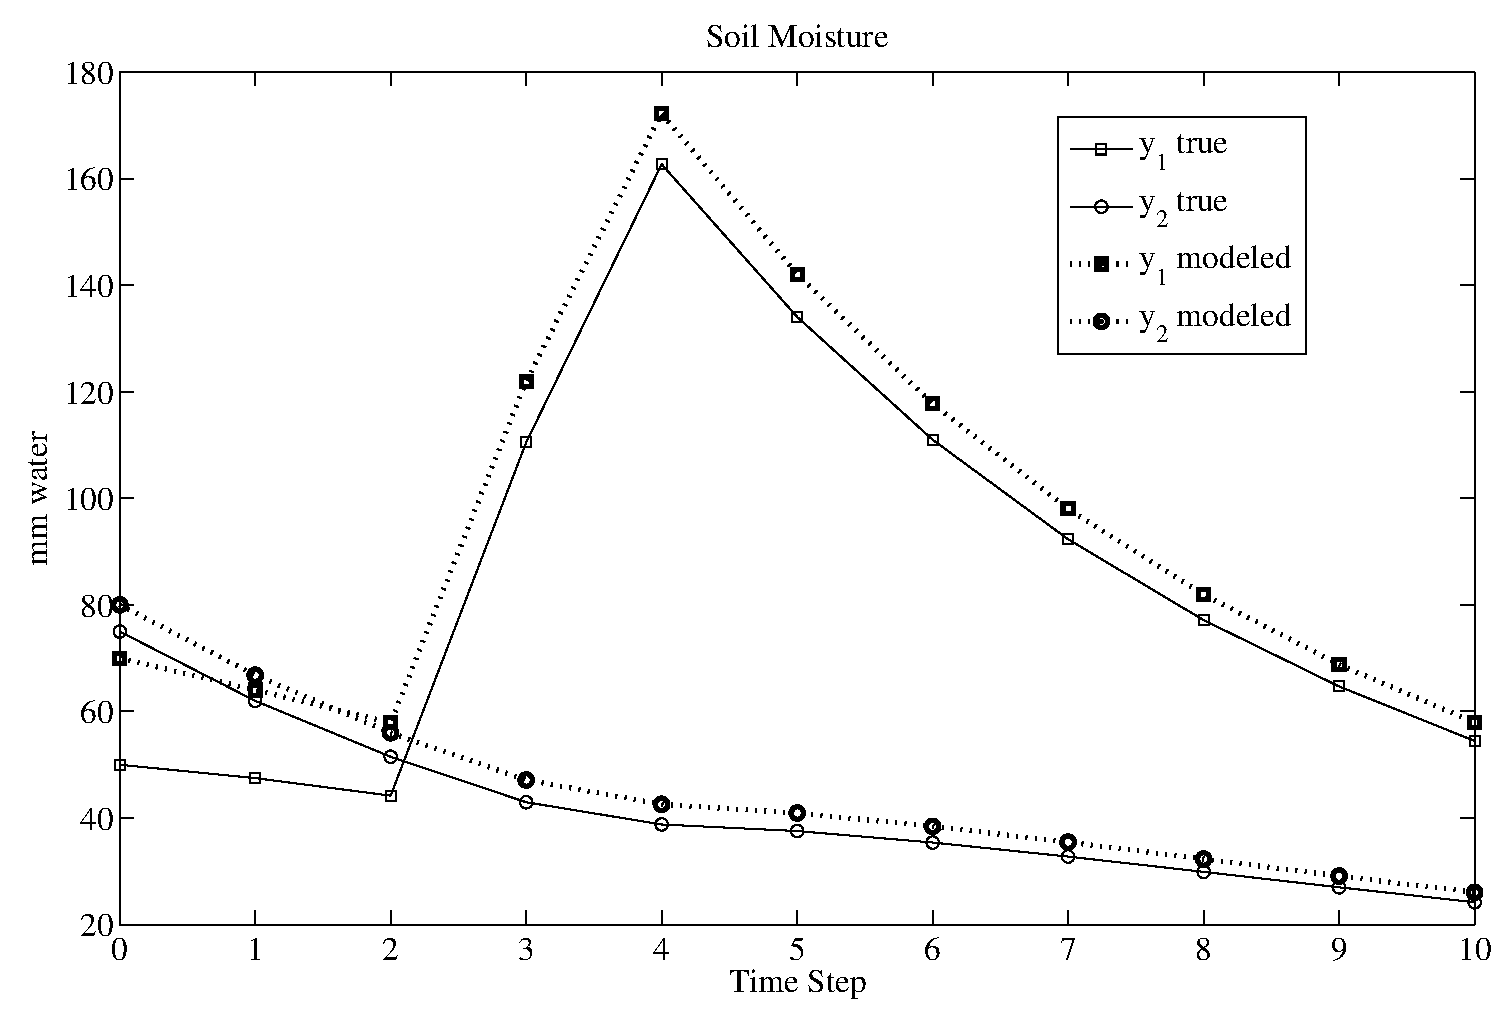
\includegraphics[width=\textwidth]{ps5figb}
        \caption{Plot of $p_X(x)=e^{-x}$}
        \label{exprnd}
\end{figure}

{\small
\begin{minipage}{\linewidth}
        \lstinputlisting[language=Matlab, caption={Monte Carlo estimation of $e^{-x}$ in MATLAB},
        basicstyle=\ttfamily, label=lst1]{ps5a.m}
\end{minipage}
}


\end{document}
